\section{Sit-to-stand Model}

\subsection{Two-Mode Hybrid Model}

The STS motion has been described as a series of phases \cite{etnyre2007}, \cite{schenkman1990}, based on observed kinematic characteristics. From a dynamic systems perspective, the action can be divided into two discrete modes: a sitting phase and a rising phase. The system dynamics switch when contact with the chair is lost. At this instant, denoted seat-off, the human transitions from a stable system to a potentially unstable system \cite{etnyre2007}. Once seat-off occurs, the system remains within the rising mode dynamics as long as the sole point of external contact is between the feet and ground. While previous work has classified STS into three or four phases, this two-mode model incorporates the only change in dynamics without further constraining the action. The hybrid and biomechanical models are show in Figure \ref{fig: dynamics}.

\subsection{Dynamical Model}

We consider a rigid-body model of the human constrained to the sagittal plane. This model consists of three segments: shank, thigh, and HAT (head-arms-trunk), with corresponding joints: ankles, knees, and hips \cite{music2008}, \cite{matthew2016}. The nonlinear dynamics of the system are represented by

\begin{equation}
\dot{x}=f(x,u) 
\end{equation}
where the states $x= \left[\theta_a, \dot{\theta_a}, \theta_k, \dot{\theta_k},\theta_h,\dot{\theta_h}, \right] \in \mathbb{R}^6$ correspond to the ankle, knee, and hip angles and angular velocities, and the inputs $u = \left[\tau_a, \tau_k, \tau_h, \right] \in \mathbb{R}^3$ correspond to the joint torques.

The equations of motion,  derived through Lagrangian dynamics, and are described by:

\begin{equation}
M\left(\theta\right)\ddot{\theta} + C(\theta, \dot{\theta})\dot{\theta} + N \left(\theta\right) = \tau
\end{equation}

where $M$ represents the inertial forces due to acceleration of the joints, $C$ represents the Coriolis and centrifugal forces, $N$ represents the potential matrix, and $\tau$ is the applied joint torques. Model parameters such as lengths, masses, COM, and COM locations along segments were selected from literature values \cite{plagenhoef1983}. 


\begin{figure}[h]
  \centering
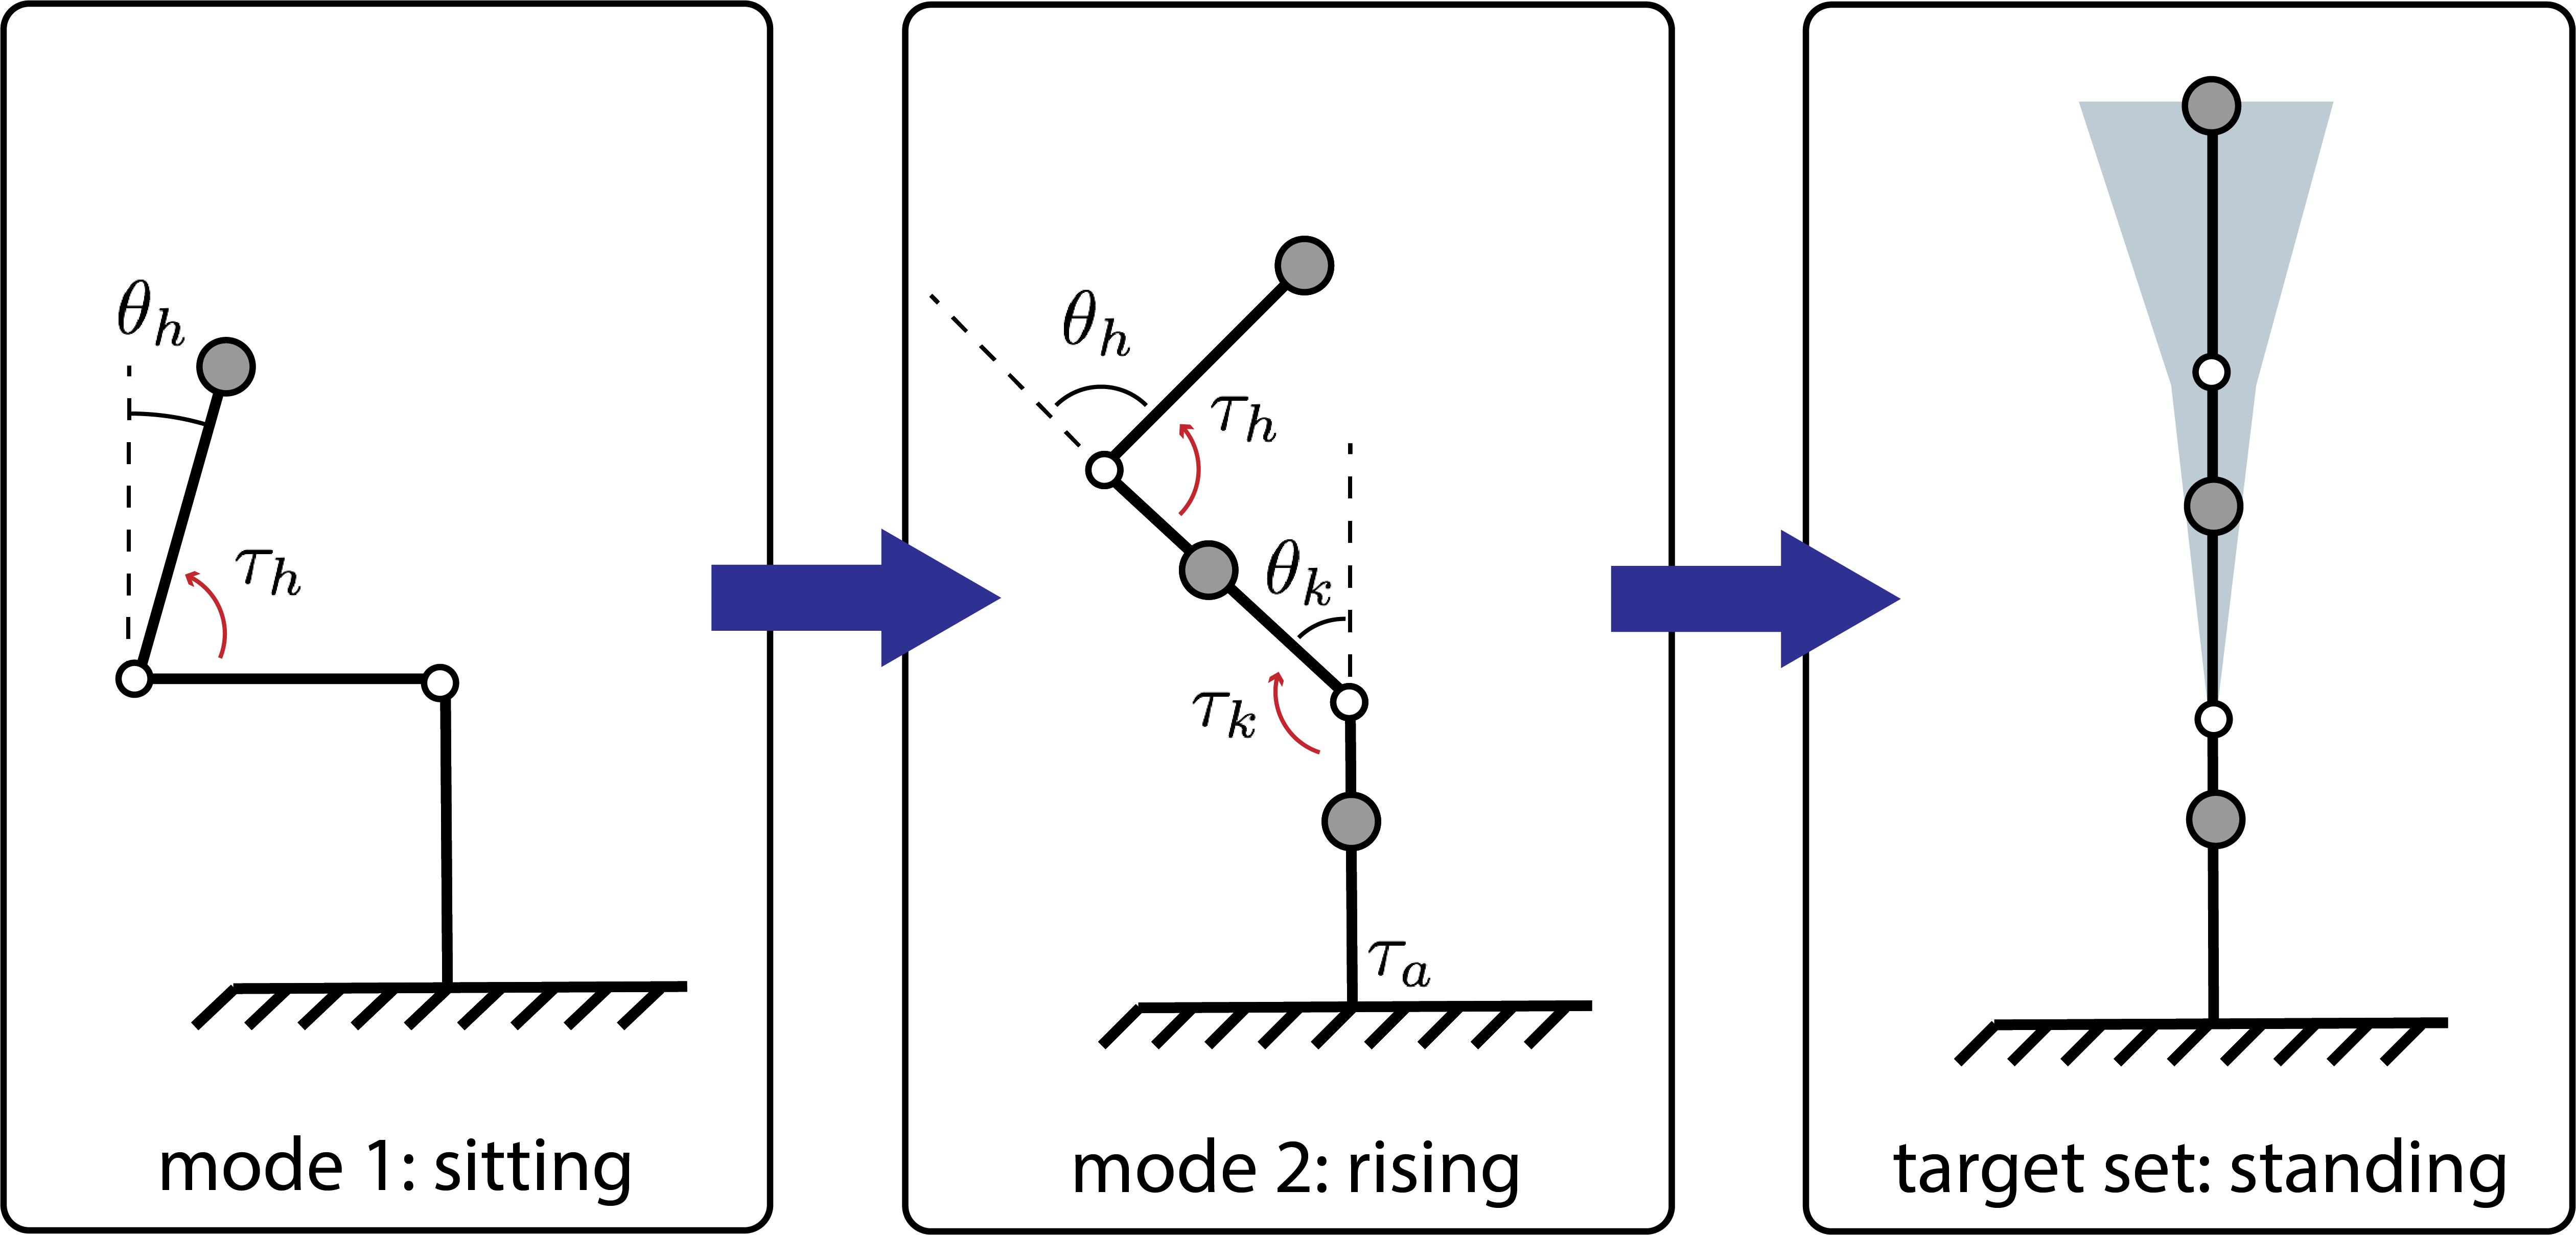
\includegraphics[width=3.4in]{figures/hybridSys.png}
\caption{Hybrid and biomechanical model of STS motion.}
  \label{fig: dynamics}
\end{figure}

Due to the computational complexity of reachability for a 6-D system, we propose a simplified model of the three segment body. During the sit-to-stand motion, the knee and hip joints exhibit greater variation in joint angle and angular velocity than the ankle joint. Thus, for initial investigation of this method, we assume the shank remains at a fixed position throughout the motion. The simplified model consists of a double inverted pendulum attached to a fixed link. Despite the limited range of motion of the ankle during STS, the joint experiences a large torque from the motion of the other body segments. We compute the resultant torque on the ankle and incorporate maximum bounds on the ankle torque when computing reachable sets. 

Alternative lower dimensional models of STS, including a telescopic pendulum\cite{papa1999} and double pendulum \cite{roberts1996} models, have been studied. However, a three-link model was selected due to its resemblance to human morphology and the direct correspondence between system inputs and joint torques. 

The above model is not representative of the seated phase due to the contact between the hips and the chair. During this phase the human bends the torso at the hip, generating momentum before leaving the seat. We model this phase as a single inverted pendulum anchored at the hip joint with the segment representing the HAT. These simplified dynamics are described by:

\begin{equation}
\ddot{\theta_h} = \frac{g}{l} \sin{\theta_h} + \frac{1}{ml^2} \tau_h
\end{equation}

%\subsection{Kinematic and Joint Torque Constraints}

Kinematic constraints on the joint angle range of motion and maximum angular velocities are set. A constraint on the maximum voluntary joint torque was placed on each joint. 
